%!TEX root = ./main.tex

%%%%%%%%%%%%%%%%%%%%%%%%%%%%%%%%%%%%%%%%%%%%%%%%%%%%%%%%%%%%%%%%
%%
%% Vorlage für Bachelor Arbeit und weitere Dokumentationen (T1000 - T3300)
%%   von Maximilian Knopf
%%   inspiriert von einer DHBW Heidenheim Vorlage, https://github.com/programonaut/latex-template
%%
%% Erstellen mitteles Kommandozeile:
%%   pdflatex main.tex
%%   biber main
%%   pdflatex main.tex
%%   pdflatex main.tex
%%%%%%%%%%%%%%%%%%%%%%%%%%%%%%%%%%%%%%%%%%%%%%%%%%%%%%%%%%%%%%%%

%!TEX root = ../main.tex

%% Literatur Resourcendateien
\newcommand{\loadbibresources}{
	\bibliography{resources/quellen.bib}
}
\newcommand{\quoteStyle}{ieee}						% Zitierstil: numeric-comp, alphabetic, ieee

%% Dokumententyp
\newcommand{\documentType}{T0\_X000}				% Laborbericht (Semester 1 & 2)
%\newcommand{\documentType}{T3\_1000}				% Praxisarbeit (Semester 1 & 2)
%\newcommand{\documentType}{T3\_2000}				% Praxisarbeit (Semester 3 & 4)
%\newcommand{\documentType}{T3\_2001}				% Praxisarbeit, Teil 1 (Semester 3, Teil 1)
%\newcommand{\documentType}{T3\_2002}				% Praxisarbeit, Teil 2 (Semester 4, Teil 2)
%\newcommand{\documentType}{T3\_3000}				% Praxisarbeit (Semester 5)
%\newcommand{\documentType}{T3\_3100}				% Studienarbeit (Semester 5 & 6)
%\newcommand{\documentType}{T3\_3300}				% Bachelor Arbeit (Semester 6)

%% Document settings
\newcommand{\documentAuthor}{Christian Manz, Niklas Hummel, Benedikt Helming}			%Autor

\newcommand{\documentTitle}{Verschiedene Prüfziffernverfahren}   	% Titel
\newcommand{\tutor}{Betreuer Ausbildungsfirma}		% Betreuer Ausbildungsfirma, nach DIN 5008
\newcommand{\evaluator}{Betreuer DHBW}				% Betreuer DHBW, nach DIN 5008
\newcommand{\documentPeriod}{Juni 20xx bis September 20xx}	% Bearbeitungszeitraum
\newcommand{\course}{TINF23ITA}						% DHBW Kurs
\newcommand{\matriculationNumberOne}{XXXXXXX (Christian Manz)}			% Autormatrikelnummer
\newcommand{\matriculationNumberTwo}{XXXXXXX (Niklas Hummel)}			% Autormatrikelnummer
\newcommand{\matriculationNumberThree}{7789253 (Benedikt Helming)}			% Autormatrikelnummer
\newcommand{\releaseDate}{30.05.2025}				% Veröffentlichungsdatum
\newcommand{\releaseLocation}{Ausbildungsfirmaort}	% Veröffentlichungsort
\newcommand{\degree}{Bachelor of Engineering}		% akademischer Grad
\newcommand{\department}{Informatik}	% Fachrichtung
\newcommand{\locationUniversity}{Stuttgart}			% DHBW Standort
\newcommand{\companyName}{Ausbildungsfirma}			% Ausbildungsfirma Name
\newcommand{\companyLocation}{12345 Ausbildungsfirmaort}	% Ausbildungsfirma Ort
%!TEX root = ../main.tex

%% Dokumentenklasse
\documentclass[%
    paper=a4,           % DIN A4
    12pt,               % Schriftgröße 12
    parskip=full,       % eine Zeile Absatzabstand
    oneside             % einseitig
    listof=totoc,		% alle Verzeichnisse in ToC einbinden
    bibliography=totoc,
    toc=listof,
    toc=chapterentrydotfill % ToC Punkte
]{scrreprt}             % KOMA Skript Report

%% Standard-Pakete
\usepackage{xstring}		            % für Stringvergleich
\usepackage[utf8]{inputenc}         	% Quelldateicodierung
\usepackage[T1]{fontenc}	            % Fontmap-Kodierung, diese wird von der pdflatex-Engine benötigt
\usepackage[english, ngerman]{babel}	% Sprache


%% ifDocType Befehlsdefinition
\newcommand{\ifDocType}[3]{%
	\IfStrEq{\documentType}{#1}{#2}{#3}%
}

%% Seiteneinstellungen
% Ränder
\usepackage[
    left=2.5cm,
    right=2.5cm,
    bottom=4cm,
    top=4cm
]{geometry}

\usepackage[onehalfspacing]{setspace}   % Zeilenabstand

% Schriftart
\usepackage{helvet}     % Arial like
\renewcommand{\familydefault}{\sfdefault}

%\usepackage{mathptmx} % Times New Roman font

% Kopf- und Fußzeile
\usepackage[headsepline=1pt, footsepline=1pt]{scrlayer-scrpage}
\renewcommand*\chapterpagestyle{scrheadings}
\pagestyle{scrheadings}
%\ifDocType{T3\_3100}{%
    % kein Logo bei T3100
%}{%
%    \lohead{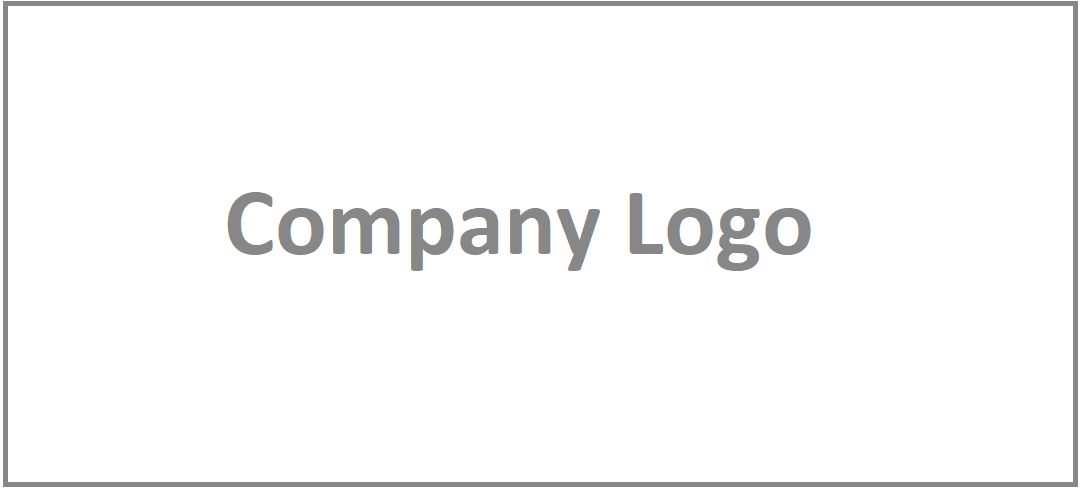
\includegraphics[height=1.5cm]{resources/images/logo-company.png}}
%}
\chead{}
\rohead{
\includegraphics[height=1.6cm]{resources/images/logo-dhbw.png}}
\newcommand{\documentTypePhrase}{%
	\IfStrEqCase{\documentType}{%
        {T0\_X000}{Hausarbeit}%
		{T3\_1000}{Projektarbeit T1000}%
		{T3\_2000}{Projektarbeit T2000}%
		{T3\_2001}{Projektarbeit T2000, Teil 1}%
		{T3\_2002}{Projektarbeit T2000, Teil 2}%
		{T3\_3000}{Projektarbeit T3000}%
		{T3\_3100}{Studienarbeit}
		{T3\_3200}{Studienarbeit}%
		{T3\_3300}{Bachelorarbeit}%
	}
}
\ifoot{\documentTypePhrase}
\cfoot{\documentAuthor}
\ofoot{Seite | \thepage}
\setlength{\marginparwidth}{2cm}

\usepackage{scrhack}    % KOMA Skript Fehlermeldung

%% Sonstige Pakete
\usepackage{todonotes}              % Todos in GROßBUCHSTABEN
\usepackage{graphicx}               % Bilder
\usepackage{svg}                    % SVG Bilder
\graphicspath{{resources/images/}}  % Standard Bilderpfad
\usepackage{subcaption}             % Mehrere Bilder/Tabllen in einer Figure
\usepackage{tikz}                   % für komplexe Bilderstellung
\usepackage{tabularx}               % Tabellen
\usepackage{pdfpages}               % PDF Dateien / Seiten
\usepackage{float}                  % Floating Darstellung
\usepackage{xcolor}                 % Farben
\usepackage{acronym}                % Abkürzungen, nur die Verwendeten: \usepackage[printonlyused]{acronym}
\usepackage{amsfonts}               % Mathematische Schriftart der American Mathematical Society
\usepackage{amsmath}                % Mathematische Schriftzeichen der American Mathematical Society
\usepackage{fancyvrb}               % [für Quelltext]
\usepackage{xurl}                   % URL Umbruch
\usepackage{pdflscape}              % Querformat
\usepackage{enumitem}               % Aufzählungsstile



% Setzen des Pfads zu Inkscape
\svgsetup{
    inkscapeexe=/Applications/Inkscape.app/Contents/MacOS/inkscape
}

%% Bibliographie
\usepackage[
	backend=biber,			% Recommended. Alternative: biblatex
	bibwarn=true,
	bibencoding=utf8,		% Wenn die .bib-Datei mit utf8 kodiert ist, sonst ascii
	sortlocale=de_DE,
	style=\quoteStyle,
]{biblatex}
\loadbibresources			% Lädt die Resourcen aus der config Datei
\newcommand{\mkbibnodate}{o\adddot J\adddot}        % o. J.
\AtEveryBibitem{\iffieldundef{year}{\restorefield{year}{\mkbibnodate}}{}}
\usepackage{csquotes}               % Zitierung mit Sprache verknüpfen

%% Querverweise und Links
\definecolor{LinkColor}{HTML}{00007A} % Farbe
\usepackage[%
    pdftitle={\documentTitle},
    pdfauthor={\documentAuthor, \documentAuthor2},
    pdfsubject={\documentType},
    pdfcreator={pdflatex, LaTeX with KOMA-Script},
    pdfpagemode=UseOutlines,
    pdfdisplaydoctitle=true,
    pdflang={de},
    colorlinks = false,
	linkcolor=LinkColor,
	citecolor=LinkColor,
	filecolor=LinkColor,
	menucolor=LinkColor,
	urlcolor=LinkColor,
	linktocpage=true,
	bookmarksnumbered=true,
    hidelinks = true
]{hyperref}

%% Quelltext
\usepackage{listings}

\definecolor{comment}{HTML}{0A943F}
\definecolor{keyword}{HTML}{184FDB}
\definecolor{background}{HTML}{F2F2F2}
\definecolor{string}{HTML}{DB9418}
\lstset{%
    backgroundcolor=\color{background},
    basicstyle=\ttfamily\footnotesize,
    breakatwhitespace=false,
    breakautoindent=true,
    breaklines=true,
    captionpos=b,
    commentstyle=\color{comment},
    keepspaces=true,
    keywordstyle=\color{keyword},
    morekeywords={var}
    numbers=left,
    numbersep=1em,
    numberstyle=\tiny,
    postbreak=\space,
    showspaces=false,
    showstringspaces=false,
    showtabs=false,
    stepnumber=1,
    stringstyle=\color{string},
    tabsize=2,
}
\lstloadlanguages{PHP,python,java,C,C++,bash}
\renewcommand\lstlistingname{Skript}
\renewcommand\lstlistlistingname{Skriptverzeichnis}
\def\lstlistingautorefname{Skript}

%% Chapter Style
\definecolor{chapterBlue}{RGB}{20,20,20}
\addtokomafont{chapter}{\color{chapterBlue}}
\addtokomafont{section}{\color{chapterBlue}}
\addtokomafont{subsection}{\color{chapterBlue}}
\addtokomafont{subsubsection}{\color{chapterBlue}}
\RedeclareSectionCommand[beforeskip=0pt,afterindent=false,afterskip=1em]{chapter}
\RedeclareSectionCommand[beforeskip=0pt,afterindent=false,afterskip=1em]{section}
\RedeclareSectionCommand[beforeskip=0pt,afterindent=false,afterskip=1em]{subsection}
\RedeclareSectionCommand[beforeskip=0pt,afterindent=false,afterskip=1em]{subsubsection}

%% Caption Style (Bsp.: Bilderunterschrift)
\addtokomafont{caption}{\small}

%% Cover Einstellungen
\title{\documentTitle}
\author{\documentAuthor1}
\author{\documentAuthor2}
\date{\releaseDate}


%% Start des Dokuments
\begin{document}
    %TODO: Liste aller TODOs, auskommentieren für die Abgabe!
    \listoftodos

    %% Titelblatt
    %!TEX root = ../main.tex

\begin{titlepage}
%% DHBW_Logo
\begin{tikzpicture}[remember picture, overlay]
	\node[anchor=north east,inner xsep=50pt, inner ysep=25pt] at (current page.north east)
	{
\includegraphics[height=2cm]{resources/images/logo-dhbw}};
\end{tikzpicture}

%% Firmen Logo
% \ifDocType{T3\_3100}{%
% 	% kein Logo bei T3100
% }{%
% 	\begin{tikzpicture}[remember picture, overlay]
% 		\node[anchor=north west,inner xsep=50pt, inner ysep=25pt] at (current page.north west)
% 		{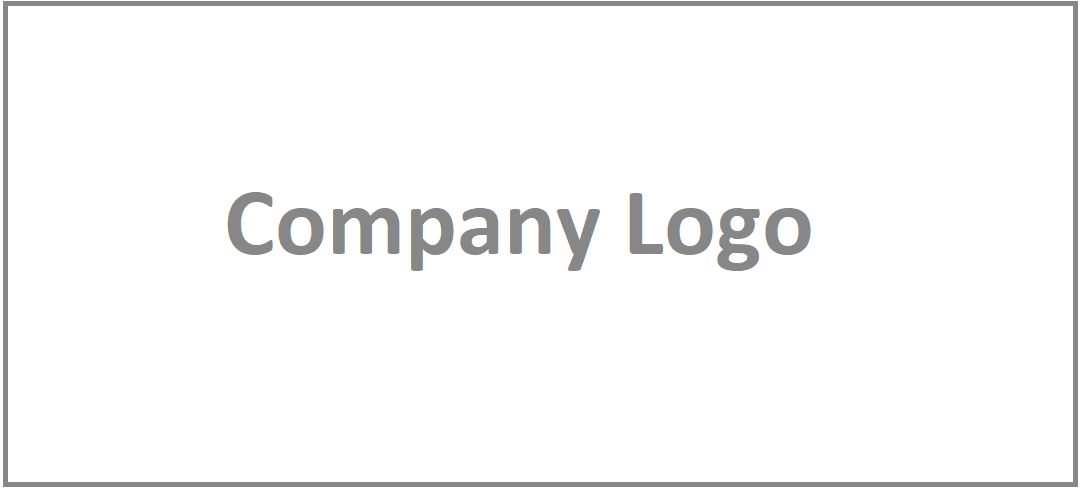
\includegraphics[height=2cm]{resources/images/logo-company}};
% 	\end{tikzpicture}
% }

\enlargethispage{20mm}
\begin{center}
	\vspace*{0mm}	{\LARGE\textbf{\documentTitle}}\\
	\vspace*{12mm}
	\vspace*{12mm}	{\large\textbf{\documentTypePhrase}}\\

	\ifDocType{T3\_3300}{
		\vspace*{12mm}	{für die Prüfung zum}\\
		\vspace*{3mm}	{\degree}\\
	}

	\vspace*{12mm}  {des Studienganges \department}\\
	\vspace*{3mm}  {an der Dualen Hochschule Baden-Württemberg \locationUniversity}\\
	\vspace*{12mm}  {von}\\
	\vspace*{3mm}  {\textbf{\documentAuthor}}\\
	\vspace*{12mm}  {\releaseDate}\\
\end{center}

\vfill

\begin{spacing}{1.2}
	\begin{tabbing}
		mmmmmmmmmmmmmmmmmmmmmmmmmm \= \kill
		%\textbf{Bearbeitungszeitraum} \> \documentPeriod \\
		\textbf{Matrikelnummer, Kurs} \> \matriculationNumberOne, \course \\
		\textbf{Matrikelnummer, Kurs} \> \matriculationNumberTwo, \course \\
		\textbf{Matrikelnummer, Kurs} \> \matriculationNumberThree, \course \\
		\ifDocType{T3\_3100}{%
			% keine Firma bei T3100
			\textbf{Betreuer der DHBW \locationUniversity} \> \evaluator
		}{%
			%\textbf{Dualer Partner} \> \companyName, \companyLocation \\
			%\textbf{Betreuer des Dualen Partners} \> \tutor \\
		}%
		\ifDocType{T3\_3300}{%
			% DHBW Gutachter 
			\textbf{Gutachter der DHBW \locationUniversity} \> \evaluator
		}{}
	\end{tabbing}
\end{spacing}
\end{titlepage}


    \pagestyle{scrheadings}
    \pagenumbering{Roman}

    %% Sperrvermerk
    \ifDocType{T3\_3100}{%
            % kein Sperrvermerk für T3100
        }{%
            %!TEX root = ../main.tex

\chapter*{Sperrvermerk}
Der Inhalt dieser Arbeit darf weder als Ganzes noch in Auszügen Personen außerhalb des Prüfungsprozesses und des Evaluationsverfahrens zugänglich gemacht werden, sofern keine anderslautende Genehmigung der Ausbildungsstätte vorliegt.

% Source: https://www.dhbw-stuttgart.de/studierendenportal/horb/elektrotechnik/studienbetrieb/praxisarbeiten/ [04.2022]

        }%

    %% Erklärung
    %!TEX root = ../main.tex

\chapter*{Erklärung}
Gemäß § 5 (3) der "`Studien- und Prüfungsordnung DHBW Technik"' vom 29. September 2017. \\
\\
Ich versichere hiermit, dass ich meine {\documentTypePhrase} mit dem Thema \textit{"`\documentTitle"'} selbstständig verfasst und keine anderen als die angegebenen Quellen und Hilfsmittel benutzt habe. Ich versichere zudem, dass die eingereichte elektronische Fassung mit der gedruckten Fassung übereinstimmt.\\
\\
\releaseLocation, \releaseDate
\vspace{2em}

\rule{6cm}{0.4pt}\\
\documentAuthor


    %% Anmerkung zum Genus des Substantivs
    %!TEX root = ../main.tex

\chapter*{Anmerkung zum Genus des Substantivs}

Auf geschlechtsspezifische Umschreibung ist hier verzichtet worden. Ein Maskulinum - wie zum Beispiel der Student - meint (selbstredend) auch weibliche und diverse Personen.


    %% Abstract
    %!TEX root = ../main.tex

\chapter*{Zusammenfassung / Abstract}

deutsch \\
\\
\textit{englisch}


    %% Inhaltsverzeichnis
    \begin{spacing}{1.2}
        \begingroup
            \setcounter{tocdepth}{2} % subchapter Anzeigetiefe
            \tableofcontents
        \endgroup
    \end{spacing}

    %% Abkürzungsverezeichnis
    %!TEX root = ../main.tex

\addchap{Abkürzungsverzeichnis}

\begin{acronym} %[ABCDEF]               % längste Abkürzung
	%\setlength{\itemsep}{-\parsep}     % Kein Abstand, kompakte Darstellung
	% Sortiere von Hand oder automatisch mit Kommandozeile (windows): sort file.txt /O file.txt

	\acro{DHBW}{Dualen Hochschule Baden-Württemberg}

\end{acronym}


    \clearpage
    \pagenumbering{arabic}

    \acresetall

    %% Inhalt
    %!TEX root = ../main.tex

\section{Einleitung}

% Prüfzifferverfahren sind ein essenzielles Werkzeug zur Sicherstellung der Datenintegrität in zahlreichen Anwendungen des täglichen Lebens. Sie dienen dazu, Eingabefehler, wie etwa Tippfehler oder Übertragungsfehler, zu erkennen und somit die Zuverlässigkeit von Daten zu erhöhen.

% In der modernen Informationsverarbeitung spielen Prüfziffern eine zentrale Rolle, beispielsweise bei der Validierung von Bankkontonummern, ISBN-Nummern für Bücher oder internationalen Standardcodes wie der IBAN. Diese Verfahren basieren auf mathematischen Prinzipien der Diskreten Mathematik und ermöglichen eine effiziente Fehlererkennung.

% Im Folgenden werden die Grundlagen der Prüfzifferverfahren erläutert, verschiedene Methoden vorgestellt und deren praktische Anwendungen diskutiert. Ziel ist es, ein tieferes Verständnis für die Funktionsweise und die Bedeutung dieser Verfahren zu vermitteln.
\chapter{Prüfzifferverfahren}


\section{ISBN}
%!TEX root = ../main.tex

\section{EAN}
%!TEX root = ../main.tex

\section{EKONS}

%!TEX root = ../main.tex

\chapter{Fazit}
Aufgabenstellung, Vorgehensweise und wesentliche Ergebnisse werden kurz und präzise dargestellt und kritisch reflektiert. Die Zusammenfassung ist eigenständig verständlich. Länge ca. 1 bis 1,5 Seiten (Problem, Ziele, Vorgehensweise, Ergebnisse und Ausblick).

\chapter{Ausblick}


%% Beispiele, können problemlos entfernt werden!
\chapter{Beispiele}
Beispiele, können problemlos entfernt werden!
\section{Literatur}
Beispiel Text \cite[S. 10]{testBuch1}
Beispiel Homepage\cite{urlId} \\

\section{Bilder}
\begin{figure}[H]
	\centering
	
\includegraphics[width=0.3\linewidth]{resources/images/logo-dhbw}
	\caption{DHBW Logo}
	\label{fig:logo-dhbw}
\end{figure}

\section{Fußnote und Abkürzung}
Fußnote\footnote{Fußnote}, \ac{DHBW}

\section{Tabelle}
\begin{table}[H]
	\centering
	\caption{Tabellenbeispiel}
	\label{tab:example}
	\begin{tabular}{|l|c|r|}
		\hline
		Spalte 1 & Spalte 2 & Spalte 3 \\
		\hline
		Zeile  &  &  \\
		\hline
		& Zeile &  \\
		\hline
		&  & Zeile \\
		\hline
		\multicolumn{2}{|r|}{Verbunden}	& nicht Verbunden \\
		\hline
	\end{tabular}
\end{table}

\section{Skript}
\lstinline[language=c]|printf("Inline Code");|
\lstinputlisting[language=python,caption={Beispiel python Skript},captionpos=t,label=scr:exanple]{resources/example-script.py}

\section{TODOs}
Text Text\todo{TODO als Randnotiz} Text
\todo[inline]{TODO als in Zeile}

\begin{landscape}
	\section{Querformat}
	Text über Tabelle \ref{tab:breitetabelle}.
	\begin{table}[H]
		\caption{Breites Tabellenbeispiel}
		\label{tab:breitetabelle}
		\centering
		\resizebox{\columnwidth}{!}{%
			\begin{tabular}{|p{10cm}|p{10cm}|p{10cm}|}
				\hline
				Sehr & breite & Tabelle \\
				\hline
				\multicolumn{3}{|c|}{Tabelle wurde in der Größe verkleinert} \\
				\hline
			\end{tabular}
		}
	\end{table}
	Text unter Tabelle \ref{tab:breitetabelle}.
\end{landscape}

\section{Auflistungen}
\begin{enumerate}
	\item Aufzählung nummeriert
\end{enumerate}
\begin{itemize}
	\item Aufzählung Stichpunkte
\end{itemize}
\begin{description}[style=nextline]
	\item[Label] Aufzählung als Beschreibung
\end{description}


    %% Literaturverzeichnis
    \printbibliography[title=Literaturverzeichnis]
    \clearpage

    %% Abbildungsverzeichnis
    \listoffigures
    \clearpage

    %% Tabellenverzeichnis
    \listoftables
    \clearpage

    %% Skriptverzeichnis
    \lstlistoflistings
    \clearpage

    %% Anhang
    \appendix
    %!TEX root = ../main.tex

\addchap{Anhang}
\begin{itemize}
	\item \ref{apx:1} Anhang 1 \dotfill{} \pageref{apx:1}
	\item \ref{apx:2} Anhang 2 \dotfill{} \pageref{apx:2}
\end{itemize}

\chapter{Anhang 1}
\label{apx:1}

\chapter{Anhang 2}
\label{apx:2}


\end{document}
